\section{Component Architecture} \label{sc:component_architecture}
\begin{figure}[H]
    \centering
    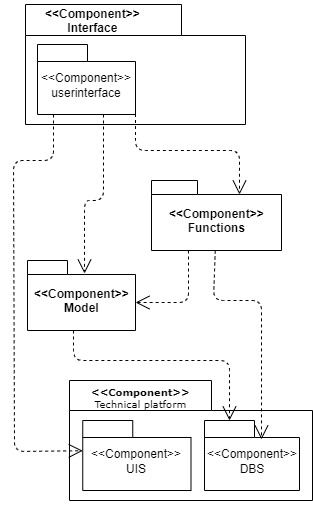
\includegraphics[width=0.6\textwidth]{figures/ComponentDiagrams/Componentdiagram.jpg}
    \caption{Component diagram for the Field Component}
    \label{fig:ComponentDesign}
\end{figure}
As seen in \autoref{fig:ComponentDesign} the architecture of the system closely resembles the "Generic Architecture Pattern" described in \citep[p 198]{OOAD}
\par
At the bottom is the database layer containing representations of the objects within the program. Above this is the model layer, which function is to convert the database representations of the objects into objects alterable by the system. These objects can then be utilized and manipulated by the functions component. At the top of the architecture, the interface is located. The interface illustrates the model component for the user and lets the user manipulate it through the function component.
\par
In the following sections, the different components will be examined and described.